
%% bare_conf.tex
%% V1.4b
%% 2015/08/26
%% by Michael Shell
%% See:
%% http://www.michaelshell.org/
%% for current contact information.
%%
%% This is a skeleton file demonstrating the use of IEEEtran.cls
%% (requires IEEEtran.cls version 1.8b or later) with an IEEE
%% conference paper.
%%
%% Support sites:
%% http://www.michaelshell.org/tex/ieeetran/
%% http://www.ctan.org/pkg/ieeetran
%% and
%% http://www.ieee.org/

%%*************************************************************************
%% Legal Notice:
%% This code is offered as-is without any warranty either expressed or
%% implied; without even the implied warranty of MERCHANTABILITY or
%% FITNESS FOR A PARTICULAR PURPOSE! 
%% User assumes all risk.
%% In no event shall the IEEE or any contributor to this code be liable for
%% any damages or losses, including, but not limited to, incidental,
%% consequential, or any other damages, resulting from the use or misuse
%% of any information contained here.
%%
%% All comments are the opinions of their respective authors and are not
%% necessarily endorsed by the IEEE.
%%
%% This work is distributed under the LaTeX Project Public License (LPPL)
%% ( http://www.latex-project.org/ ) version 1.3, and may be freely used,
%% distributed and modified. A copy of the LPPL, version 1.3, is included
%% in the base LaTeX documentation of all distributions of LaTeX released
%% 2003/12/01 or later.
%% Retain all contribution notices and credits.
%% ** Modified files should be clearly indicated as such, including  **
%% ** renaming them and changing author support contact information. **
%%*************************************************************************


% *** Authors should verify (and, if needed, correct) their LaTeX system  ***
% *** with the testflow diagnostic prior to trusting their LaTeX platform ***
% *** with production work. The IEEE's font choices and paper sizes can   ***
% *** trigger bugs that do not appear when using other class files.       ***                          ***
% The testflow support page is at:
% http://www.michaelshell.org/tex/testflow/



\documentclass[conference]{IEEEtran}
% Some Computer Society conferences also require the compsoc mode option,
% but others use the standard conference format.
%
% If IEEEtran.cls has not been installed into the LaTeX system files,
% manually specify the path to it like:
% \documentclass[conference]{../sty/IEEEtran}





% Some very useful LaTeX packages include:
% (uncomment the ones you want to load)


% *** MISC UTILITY PACKAGES ***
%
%\usepackage{ifpdf}
% Heiko Oberdiek's ifpdf.sty is very useful if you need conditional
% compilation based on whether the output is pdf or dvi.
% usage:
% \ifpdf
%   % pdf code
% \else
%   % dvi code
% \fi
% The latest version of ifpdf.sty can be obtained from:
% http://www.ctan.org/pkg/ifpdf
% Also, note that IEEEtran.cls V1.7 and later provides a builtin
% \ifCLASSINFOpdf conditional that works the same way.
% When switching from latex to pdflatex and vice-versa, the compiler may
% have to be run twice to clear warning/error messages.






% *** CITATION PACKAGES ***
%
%\usepackage{cite}
% cite.sty was written by Donald Arseneau
% V1.6 and later of IEEEtran pre-defines the format of the cite.sty package
% \cite{} output to follow that of the IEEE. Loading the cite package will
% result in citation numbers being automatically sorted and properly
% "compressed/ranged". e.g., [1], [9], [2], [7], [5], [6] without using
% cite.sty will become [1], [2], [5]--[7], [9] using cite.sty. cite.sty's
% \cite will automatically add leading space, if needed. Use cite.sty's
% noadjust option (cite.sty V3.8 and later) if you want to turn this off
% such as if a citation ever needs to be enclosed in parenthesis.
% cite.sty is already installed on most LaTeX systems. Be sure and use
% version 5.0 (2009-03-20) and later if using hyperref.sty.
% The latest version can be obtained at:
% http://www.ctan.org/pkg/cite
% The documentation is contained in the cite.sty file itself.






% *** GRAPHICS RELATED PACKAGES ***
%
\ifCLASSINFOpdf
   \usepackage[pdftex]{graphicx}
  % declare the path(s) where your graphic files are
  % \graphicspath{{../pdf/}{../jpeg/}}
  % and their extensions so you won't have to specify these with
  % every instance of \includegraphics
  % \DeclareGraphicsExtensions{.pdf,.jpeg,.png}
\else
  % or other class option (dvipsone, dvipdf, if not using dvips). graphicx
  % will default to the driver specified in the system graphics.cfg if no
  % driver is specified.
  % \usepackage[dvips]{graphicx}
  % declare the path(s) where your graphic files are
  % \graphicspath{{../eps/}}
  % and their extensions so you won't have to specify these with
  % every instance of \includegraphics
  % \DeclareGraphicsExtensions{.eps}
\fi
% graphicx was written by David Carlisle and Sebastian Rahtz. It is
% required if you want graphics, photos, etc. graphicx.sty is already
% installed on most LaTeX systems. The latest version and documentation
% can be obtained at: 
% http://www.ctan.org/pkg/graphicx
% Another good source of documentation is "Using Imported Graphics in
% LaTeX2e" by Keith Reckdahl which can be found at:
% http://www.ctan.org/pkg/epslatex
%
% latex, and pdflatex in dvi mode, support graphics in encapsulated
% postscript (.eps) format. pdflatex in pdf mode supports graphics
% in .pdf, .jpeg, .png and .mps (metapost) formats. Users should ensure
% that all non-photo figures use a vector format (.eps, .pdf, .mps) and
% not a bitmapped formats (.jpeg, .png). The IEEE frowns on bitmapped formats
% which can result in "jaggedy"/blurry rendering of lines and letters as
% well as large increases in file sizes.
%
% You can find documentation about the pdfTeX application at:
% http://www.tug.org/applications/pdftex





% *** MATH PACKAGES ***
%
%\usepackage{amsmath}
% A popular package from the American Mathematical Society that provides
% many useful and powerful commands for dealing with mathematics.
%
% Note that the amsmath package sets \interdisplaylinepenalty to 10000
% thus preventing page breaks from occurring within multiline equations. Use:
%\interdisplaylinepenalty=2500
% after loading amsmath to restore such page breaks as IEEEtran.cls normally
% does. amsmath.sty is already installed on most LaTeX systems. The latest
% version and documentation can be obtained at:
% http://www.ctan.org/pkg/amsmath





% *** SPECIALIZED LIST PACKAGES ***
%
%\usepackage{algorithmic}
% algorithmic.sty was written by Peter Williams and Rogerio Brito.
% This package provides an algorithmic environment fo describing algorithms.
% You can use the algorithmic environment in-text or within a figure
% environment to provide for a floating algorithm. Do NOT use the algorithm
% floating environment provided by algorithm.sty (by the same authors) or
% algorithm2e.sty (by Christophe Fiorio) as the IEEE does not use dedicated
% algorithm float types and packages that provide these will not provide
% correct IEEE style captions. The latest version and documentation of
% algorithmic.sty can be obtained at:
% http://www.ctan.org/pkg/algorithms
% Also of interest may be the (relatively newer and more customizable)
% algorithmicx.sty package by Szasz Janos:
% http://www.ctan.org/pkg/algorithmicx




% *** ALIGNMENT PACKAGES ***
%
%\usepackage{array}
% Frank Mittelbach's and David Carlisle's array.sty patches and improves
% the standard LaTeX2e array and tabular environments to provide better
% appearance and additional user controls. As the default LaTeX2e table
% generation code is lacking to the point of almost being broken with
% respect to the quality of the end results, all users are strongly
% advised to use an enhanced (at the very least that provided by array.sty)
% set of table tools. array.sty is already installed on most systems. The
% latest version and documentation can be obtained at:
% http://www.ctan.org/pkg/array


% IEEEtran contains the IEEEeqnarray family of commands that can be used to
% generate multiline equations as well as matrices, tables, etc., of high
% quality.




% *** SUBFIGURE PACKAGES ***
%\ifCLASSOPTIONcompsoc
%  \usepackage[caption=false,font=normalsize,labelfont=sf,textfont=sf]{subfig}
%\else
%  \usepackage[caption=false,font=footnotesize]{subfig}
%\fi
% subfig.sty, written by Steven Douglas Cochran, is the modern replacement
% for subfigure.sty, the latter of which is no longer maintained and is
% incompatible with some LaTeX packages including fixltx2e. However,
% subfig.sty requires and automatically loads Axel Sommerfeldt's caption.sty
% which will override IEEEtran.cls' handling of captions and this will result
% in non-IEEE style figure/table captions. To prevent this problem, be sure
% and invoke subfig.sty's "caption=false" package option (available since
% subfig.sty version 1.3, 2005/06/28) as this is will preserve IEEEtran.cls
% handling of captions.
% Note that the Computer Society format requires a larger sans serif font
% than the serif footnote size font used in traditional IEEE formatting
% and thus the need to invoke different subfig.sty package options depending
% on whether compsoc mode has been enabled.
%
% The latest version and documentation of subfig.sty can be obtained at:
% http://www.ctan.org/pkg/subfig




% *** FLOAT PACKAGES ***
%
%\usepackage{fixltx2e}
% fixltx2e, the successor to the earlier fix2col.sty, was written by
% Frank Mittelbach and David Carlisle. This package corrects a few problems
% in the LaTeX2e kernel, the most notable of which is that in current
% LaTeX2e releases, the ordering of single and double column floats is not
% guaranteed to be preserved. Thus, an unpatched LaTeX2e can allow a
% single column figure to be placed prior to an earlier double column
% figure.
% Be aware that LaTeX2e kernels dated 2015 and later have fixltx2e.sty's
% corrections already built into the system in which case a warning will
% be issued if an attempt is made to load fixltx2e.sty as it is no longer
% needed.
% The latest version and documentation can be found at:
% http://www.ctan.org/pkg/fixltx2e


%\usepackage{stfloats}
% stfloats.sty was written by Sigitas Tolusis. This package gives LaTeX2e
% the ability to do double column floats at the bottom of the page as well
% as the top. (e.g., "\begin{figure*}[!b]" is not normally possible in
% LaTeX2e). It also provides a command:
%\fnbelowfloat
% to enable the placement of footnotes below bottom floats (the standard
% LaTeX2e kernel puts them above bottom floats). This is an invasive package
% which rewrites many portions of the LaTeX2e float routines. It may not work
% with other packages that modify the LaTeX2e float routines. The latest
% version and documentation can be obtained at:
% http://www.ctan.org/pkg/stfloats
% Do not use the stfloats baselinefloat ability as the IEEE does not allow
% \baselineskip to stretch. Authors submitting work to the IEEE should note
% that the IEEE rarely uses double column equations and that authors should try
% to avoid such use. Do not be tempted to use the cuted.sty or midfloat.sty
% packages (also by Sigitas Tolusis) as the IEEE does not format its papers in
% such ways.
% Do not attempt to use stfloats with fixltx2e as they are incompatible.
% Instead, use Morten Hogholm'a dblfloatfix which combines the features
% of both fixltx2e and stfloats:
%
% \usepackage{dblfloatfix}
% The latest version can be found at:
% http://www.ctan.org/pkg/dblfloatfix




% *** PDF, URL AND HYPERLINK PACKAGES ***
%
\usepackage{url}
% url.sty was written by Donald Arseneau. It provides better support for
% handling and breaking URLs. url.sty is already installed on most LaTeX
% systems. The latest version and documentation can be obtained at:
% http://www.ctan.org/pkg/url
% Basically, \url{my_url_here}.




% *** Do not adjust lengths that control margins, column widths, etc. ***
% *** Do not use packages that alter fonts (such as pslatex).         ***
% There should be no need to do such things with IEEEtran.cls V1.6 and later.
% (Unless specifically asked to do so by the journal or conference you plan
% to submit to, of course. )


% correct bad hyphenation here
\hyphenation{op-tical net-works semi-conduc-tor}


\begin{document}
%
% paper title
% Titles are generally capitalized except for words such as a, an, and, as,
% at, but, by, for, in, nor, of, on, or, the, to and up, which are usually
% not capitalized unless they are the first or last word of the title.
% Linebreaks \\ can be used within to get better formatting as desired.
% Do not put math or special symbols in the title.
\title{Local Optimizations in Eclipse QVTc and QVTr using the Micro-Mapping Model of Computation}


% author names and affiliations
% use a multiple column layout for up to three different
% affiliations
\author{\IEEEauthorblockN{Edward D. Willink}
\IEEEauthorblockA{Willink Transformations Ltd.\\
Reading, United Kingdom\\
Email: ed\_at\_willink.me.uk}}

% conference papers do not typically use \thanks and this command
% is locked out in conference mode. If really needed, such as for
% the acknowledgment of grants, issue a \IEEEoverridecommandlockouts
% after \documentclass

% for over three affiliations, or if they all won't fit within the width
% of the page, use this alternative format:
% 
%\author{\IEEEauthorblockN{Michael Shell\IEEEauthorrefmark{1},
%Homer Simpson\IEEEauthorrefmark{2},
%James Kirk\IEEEauthorrefmark{3}, 
%Montgomery Scott\IEEEauthorrefmark{3} and
%Eldon Tyrell\IEEEauthorrefmark{4}}
%\IEEEauthorblockA{\IEEEauthorrefmark{1}School of Electrical and Computer Engineering\\
%Georgia Institute of Technology,
%Atlanta, Georgia 30332--0250\\ Email: see http://www.michaelshell.org/contact.html}
%\IEEEauthorblockA{\IEEEauthorrefmark{2}Twentieth Century Fox, Springfield, USA\\
%Email: homer@thesimpsons.com}
%\IEEEauthorblockA{\IEEEauthorrefmark{3}Starfleet Academy, San Francisco, California 96678-2391\\
%Telephone: (800) 555--1212, Fax: (888) 555--1212}
%\IEEEauthorblockA{\IEEEauthorrefmark{4}Tyrell Inc., 123 Replicant Street, Los Angeles, California 90210--4321}}




% use for special paper notices
%\IEEEspecialpapernotice{(Invited Paper)}




% make the title area
\maketitle

% As a general rule, do not put math, special symbols or citations
% in the abstract
\begin{abstract}
The OMG QVT FAS\footnote{Object Management Group Query/View/Transformation Final Adopted Specification.} was the result of, perhaps premature, enthusiasm to standardize the fledging model transformation community. The Eclipse implementation of the QVTo language prospers but the initial implementations of the declarative QVTr language had poor performance and have faded away. Perhaps it is time to consign QVTc and QVTr to the dustbin of misguided initiatives. Alternatively, in this paper we show how metamodel-driven analysis and a disciplined Model of Computation support fulfilment of the original aspirations.
\end{abstract}

\begin{IEEEkeywords}
Graph Optimization; QVT; QVTc; QVTr; Micro-Mapping; Model of Computation
\end{IEEEkeywords}



% For peer review papers, you can put extra information on the cover
% page as needed:
% \ifCLASSOPTIONpeerreview
% \begin{center} \bfseries EDICS Category: 3-BBND \end{center}
% \fi
%
% For peerreview papers, this IEEEtran command inserts a page break and
% creates the second title. It will be ignored for other modes.
\IEEEpeerreviewmaketitle



\section{Introduction}

The OMG QVT specification~\cite{QVT-1.3} was planned as the standard solution to model transformation problems. The Request for Proposals in 2002 stimulated 8 responses that eventually coalesced as a merged submission in 2005 for three languages.

The QVTo language provides an imperative style of transformation. It stimulated two useful implementations, SmartQVT and Eclipse QVTo. %Only Eclipse QVTo is still maintained.

The QVTr language provides a rich declarative style of transformation. It stimulated two implementations. However ModelMorf never progressed beyond beta releases. 
%It is no longer available.
Medini QVT had disappointing performance and is not maintained.

The QVTc language provides a much simpler declarative capability that was intended to provide a common core for the other languages. However there has never been a QVTc implementation since the Compuware prototype was not updated to track the evolution of the merged QVT submission.

The Eclipse QVTd project~\cite{Eclipse-QVTd} extended and enhanced the Eclipse OCL~\cite{Eclipse-OCL} framework to provide QVTc and QVTr editors, but until now provided no execution capability. This paper introduces the Micro-Mapping and its Model of Computation that underpins the production of efficient schedules and describes local Micro-Mapping optimizations.

In Section~\ref{Architecture} we briefly describe the Eclipse QVTd architecture in order to provide the application context for Micro-Mappings. In Section~\ref{Declarative Transformation Execution} we consider how a declarative transformation is executed to motivate the Micro-Mapping Model of Computation in Section~\ref{The Micro-Mapping Model of Computation}. A running example is presented in Section \ref{Micro-Mapping Example} and resumed in Section \ref {Local Optimization}. Results from the example appear in Section~\ref{Results} demonstrating some scalability and code generation speed-ups. Section~\ref{Related Work} summarizes some related work and Section~\ref{Conclusions} concludes.

\section{Progressive Transformation Architecture}\label{Architecture}

The Eclipse QVTd architecture `solves' the problem of implementing a triple language specification by introducing Yet Another Three QVT Languages\cite{ya3qvt} (QVTu, QVTm and QVTi). Figure \ref{fig:architecture} shows that a further QVTs is useful.

\begin{figure}[h]
	\centering
	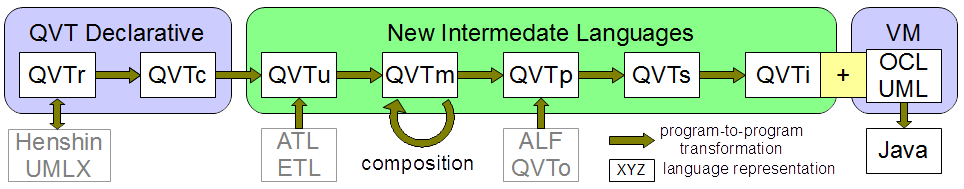
\includegraphics[width=0.5\textwidth]{QVThorizontalAlphabet.png}
	\caption{Progressive transformation approach for Declarative QVT.}
	\label{fig:architecture}
\end{figure}

\subsubsection{QVTr2QVTc} the incomplete RelToCore transformation from the QVT specification. This is still a work in progress.

\subsubsection{QVTc2QVTu} creates a Unidirectional transformation without the bloat for the unwanted directions.

\subsubsection{QVTu2QVTm} creates a Minimal transformation free from the complexities of mapping refinement and composition.

\subsubsection{QVTm2QVTs} converts to a graphical form suitable for static Scheduling analyses.

\subsubsection{QVTs2QVTs} rewrites as Micro-Mappings to avoid livelock / deadlock hazards and establishes an efficient Schedule.

\subsubsection{QVTs2QVTi} serializes to an Imperative form for direct execution by the QVTi interpreter that extends the OCL Virtual Machine. Alternatively an extension of the OCL code generator produces Java code with one outer class per transformation and a function or inner class per compound Micro-Mapping. The generated Java code bypasses many of the overheads of interpreted execution or dynamic EMF.

In this paper we concentrate on the local schedule analyses and optimizations that result in the creation of Micro-Mappings at the start of the QVTs2QVTs transformation.

\section{Declarative Transformation Execution}\label{Declarative Transformation Execution}

An imperative transformation author provides the control strategy that the transformation tooling must use in order to execute the transformation. The performance is governed by the quality of the programmed control strategy and the ability of the transformation tool to implement what it has been instructed to do. The accuracy is totally dependent on unchecked assertions that required function inputs are ready.

In contrast, a declarative transformation just expresses a truth that relates the output models to the input models. The truth can be demonstrated after the transformation completes, but how the constraints that express the truth are executed may not be obvious. A declarative transformation therefore requires less programming\footnote{Declarative transformation authors must learn to express the truth of what must happen rather than the mechanism by which it is done.}, but declarative transformation tooling must discover an appropriate control strategy to establish the required truth. This provides an opportunity to provide inherently accurate solutions that are faster than those for imperative transformation languages. But it also requires substantial compilation effort to avoid poor quality solutions.

\subsection{Commit-Actions, Micro-Mappings and Naive Scheduling}

The result of a transformation is one or more intermediate or output models each of which may be rendered as a UML Instance Diagram with Class-typed nodes for the model elements and Property-typed edges for their relationships. A diagram may be drawn one node or edge at a time, nodes before edges. A declarative transformation may therefore execute one commit action at a time, where a commit action either creates a node or assigns an edge. The type of object created, or the value assigned by the commit-action is computed from zero or more objects or values that must be ready for use. We therefore wrap the commit-action up inside a primitive Micro-Mapping to include the input parameters, predicates and computations that influence the commit-action. A primitive Micro-Mapping is therefore similar to the mapping or rule or relation of declarative transformation languages, but is constrained to a single commit-action. The correct sequence of primitive Micro-Mapping invocations can be found by a naive polling scheduler executing each primitive Micro-Mapping  once after checking that all the objects and values that the Micro-Mapping depends upon are ready and compatible.

\begin{flushleft}
~~~~Retry loop \{~~~~~~~~~~~~~~~-- until finished\\
~~~~~~~~Invocation loop \{~~~~~-- all Micro-Mappings\\
~~~~~~~~~~~~Object loops \{~~~~~-- all object/parameter pairs\\
~~~~~~~~~~~~~~~~Compatibility guard\\
~~~~~~~~~~~~~~~~Repetition guard\\
~~~~~~~~~~~~~~~~Validity guard\\
~~~~~~~~~~~~~~~~Execute Micro-Mapping\\
~~~~~~~~~~~~~~~~Create repetition memento\\
~~~~~~~~~~~~\}\\
~~~~~~~~\}\\
~~~~\}\\
\end{flushleft}

This is hideously inefficient. The many executions, wrapped in at least three loops, with guards and mementos contrast poorly to the simple linear `loop' nests of imperative programs. Fortunately there are many static analyses that we can perform on a declarative transformation in conjunction with its metamodels to tame the naive polling scheduler.

\subsection{Global Micro-Mapping Optimizations}\label{Global Micro-Mapping Optimizations}

\subsubsection{Retries}Most retries can be avoided by executing Micro-Mappings in a sensible order exploiting producer/consumer relationships between mappings. Where retries are necessary, they can be a result of useful progress rather than naive polling.

\subsubsection{Invocations}Dead Micro-Mappings can be eliminated, but most Micro-Mappings will normally be required. The invocation loop cannot be eliminated, rather it should be effectively sequenced.

\subsubsection{Objects}Considering all permutations of all objects with respect to all parameters is unnecessary; the metamodel provides a strong type system that should allow only type compatible permutations to be considered. In particular a Micro-Mapping that produces some type can be followed by a Micro-Mapping that consumes that type.

Once Micro-Mappings are scheduled in a deterministic order, many of the guards can be optimized away and many of the invocation mementos eliminated since only a single invocation is possible.

The above optimizations are global. In this paper we concentrate on the utility of Micro-Mappings and local optimizations that facilitate the overall global optimizations. Global optimization will be described in another paper.
  
\subsection{Local Micro-Mapping Optimizations}

Permuting candidate objects and parameters can lead to very poor performance, typically a two parameter quadratic search, but worse for more parameters. In this paper we will see how Micro-Mapping analysis in conjunction with the metamodel relationships enables most Micro-Mappings to be reduced to a single parameter avoiding the very poor performance. %Further analysis of something-to-many relationships enables most of the residual multiple parameter Micro-Mappings to be reduced to a single parameter with local loops leading to linear performance with respect to the number of output model elements. It appears that only genuinely Cartesian problems need multiple parameters and non-linear performance. 

\subsection{Compound Micro-Mappings}

Declarative transformation languages do not require each commit-action to be separately programmed, rather mappings (or rules or relations) aggregate one or more commit-actions as an output object pattern related to an input object pattern. These patterns impose dependencies on the availability of source objects, and guard conditions upon their suitability. In the following example we will see how the failure to distinguish between primitive and compound Micro-Mappings causes trouble for some transformation languages and conversely how recognizing the distinction enables Eclipse QVTd to give good performance.

\section{Micro-Mapping Example}\label{Micro-Mapping Example}

We will consider a very simple example that has some interesting difficulties. We will transform a model comprising a DoublyLinkedList that owns a ring of Elements into another DoublyLinkedList that owns a copied ring of Elements with the order of elements in the ring reversed. The metamodel is shown in Figure \ref{fig:DoublyLinkedListMM}. Since we use models rather than Java Objects, the complexities of maintaining bidirectional linkages are subsumed by the metamodel bidirectional relationships.

\begin{figure}[h]
	\centering
	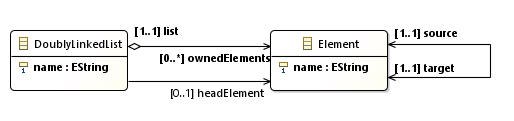
\includegraphics[width=0.5\textwidth]{doublylinkedlist.png}
	\caption{Example Metamodel - Doubly Linked List.}
	\label{fig:DoublyLinkedListMM}
\end{figure}

\subsection{ATL Implementation}

The transformation is sufficiently simple to show the full unidirectional implementation in ATL in Figure \ref{fig:Forward2Reverse-ATL}. The transformation requires two rules. list2list declares the mapping from the forwardList input to the reverseList output, populating its name and headElement. element2element populates a reverseElement from a forwardElement. The target to source assignment performs the reversal.

\begin{figure}[h]
	\centering
	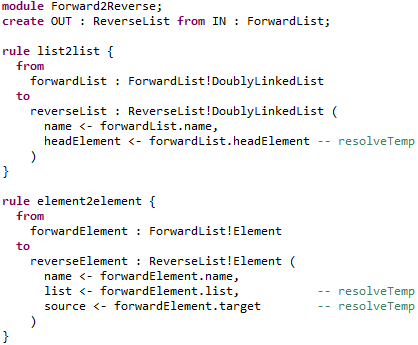
\includegraphics[width=0.45\textwidth]{Forward2Reverse-ATL.png}
	\caption{Example transformation in ATL.}
	\label{fig:Forward2Reverse-ATL}
\end{figure}

The exposition is particularly easy in ATL where the implicit resolution of the new-headElement from the old-headElement is done automatically. The commented lines show where an implicit resolution is performed.

Careful study of the transformation reveals that full execution of list2list requires that element2element has previously created the new headElement and that full execution of element2element requires that list2list has previously created the new reverseList. Further study reveals that full execution of element2element requires that another execution of element2element has created its new source which recurses to require that yet another execution of element2element has created the new source's source. The recursion terminates with full execution of element2element requiring that element2element has already created its reverseElement. These dependencies are obscure, cyclic and seemingly insoluble.

\subsection{QVTr Implementation}

Figure \ref{fig:List2List-QVTr} provides the bidirectional QVTr equivalent of ATL's unidirectional list2list rule. The asymmetric to/from patterns are replaced by symmetric forward/reverse patterns. forwardList.headElement and reverseList.headElement are explicitly co-ordinated by a when clause rather than syntax sugar.

\begin{figure}[h]
	\centering
	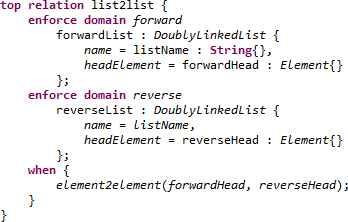
\includegraphics[width=0.4\textwidth]{List2List-QVTr.png}
	\caption{Example list2list Mapping in QVTr.}
	\label{fig:List2List-QVTr}
\end{figure}


\subsection{QVTs Colored Mapping Instance Diagrams}

Once a forward execution direction has been selected, the Eclipse QVTr/QVTc tooling provides the UML-like QVTs rendering of the mappings shown in Figures \ref{fig:List2List-QVTs} and \ref{fig:Element2Element-QVTs}.

\begin{figure}[h]
	\centering
	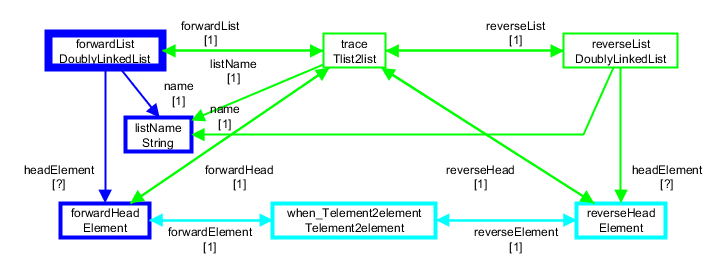
\includegraphics[width=0.45\textwidth]{List2List-QVTs.png}
	\caption{list2list Mapping in QVTs.}
	\label{fig:List2List-QVTs}
\end{figure}

\begin{figure}[h]
	\centering
	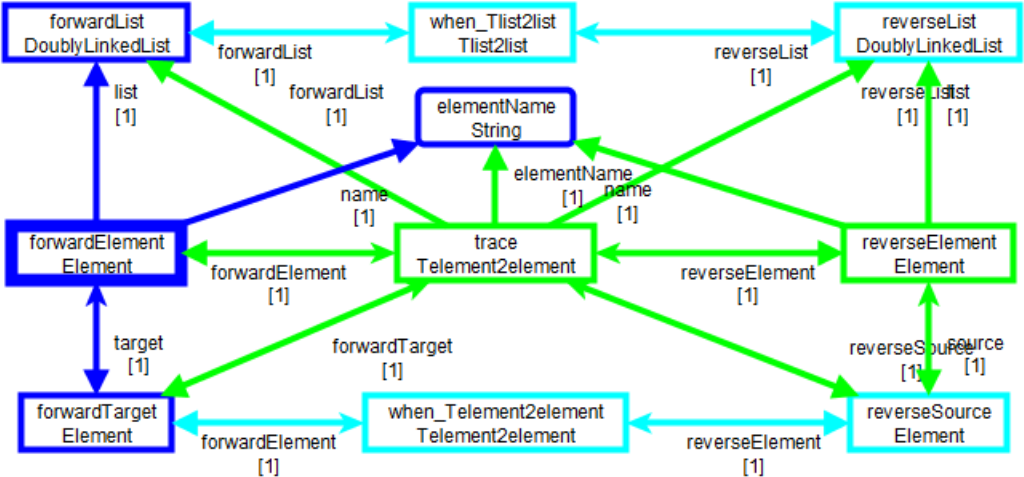
\includegraphics[width=0.45\textwidth]{Element2Element-QVTs.png}
	\caption{element2element Mapping in QVTs.}
	\label{fig:Element2Element-QVTs}
\end{figure}

Rectangles represent Class instances with an instance name above a Class name. Rounded rectangles similarly represent shared DataType values.

Edges show directed Properties with  name and cardinality. The left hand edge depicts the navigation constraint \verb|forwardHead = forwardList.headElement|. Arrows show something-to-one navigation paths.

Colors show the validity of each part of the mapping.

\begin{itemize}
\item BLACK - model elements that are constant
\item BLUE - model elements that form part of the input model
\item CYAN - model elements required before execution
\item GREEN - model elements created by execution
\end{itemize} 

The diagrams are created automatically; only the layout has been enhanced manually. On the left hand side BLUE elements show the input sub-pattern. On the right hand side there is a corresponding output sub-pattern. QVTc and QVTr differ from other transformation languages through the use of explicit model elements to trace the execution of each mapping. There is therefore a column of trace elements directly connected to each other and to the side patterns. Since in OCL, which QVT extends, all unidirectional navigations are bidirectionally navigable, the trace elements are navigable from the sides and so left, trace and right are unified in an overall pattern. In other transformation languages the trace is an implementation detail requiring irregular language constructs to exploit it.

\section{The Micro-Mapping Model of Computation}\label{The Micro-Mapping Model of Computation}

Diagrams or rather graphs of nodes and edges provide a useful way to understand systems and also computations. But as demonstrated by the Ptolemy group, diagrams only become really useful once there is a Model of Computation \cite{moc} to define the semantics of information flow along the edges.% We must therefore define the Model of Computation for a Micro-Mapping.

A Mapping provides a pattern of constraints that are all satisfied once the Mapping has been executed. It therefore defines the overall truth. In QVTs, colors are used to support intermediate partial truths. The BLACK color identifies compile-time truth. The BLUE is true after input models are loaded. The GREEN  is true as a consequence of the truth of BLACK, BLUE and CYAN elements. Partial truths evolve as successively more BLACK then BLUE then CYAN then GREEN elements are resolved.

A Mapping involving more than one GREEN element may not be executable since the multiple GREEN-after-CYAN constraints in one Mapping may deadlock with respect to an inverse ordering in another Mapping. 

\subsection{Partitioning, Primitive Micro-Mappings}\label{Partitioning}\label{Primitive Micro-Mapping}

Primitive Micro-Mappings avoid the deadlock hazard by partitioning the Mapping into multiple primitive Micro-Mappings each with a single GREEN element. This gives a very simple execution semantic; nothing happens until all CYAN elements are available, then execution proceeds uneventfully. When partitioning a Mapping into primitive Micro-Mappings, the chosen GREEN element may depend on other GREEN elements. These other GREEN elements are recolored CYAN since they are prerequisites of the chosen GREEN element. This is rather easy graphically.  

\subsection{Local Merging, Compound Micro-Mappings}\label{Local Merging}\label{Compound Micro-Mapping}

Partitioning a Mapping such as Figure \ref{fig:List2List-QVTs} leads to nine primitive Micro-Mappings to eliminate the deadlock hazards. Primitive Micro-Mappings that share the same dependencies may be merged to form a compound Micro-Mapping without losing the string properties of a primitive Micro-Mapping.

\subsection{Typed Nodes}

Each node is typed by a metamodel Class and has an instance name distinguishing its role in the overall pattern. 

\subsection{Typed Directed Edges}

Each edge is typed by a metamodel Property that defines its name, direction and cardinality, which must be something-to-one. Consequently whenever a source object exists, a target object must form part of the final truth.
%The converse is not necessarily true, but 
Wherever the metamodel defines a something-to-one opposite relationship, the opposite edge is added to the Micro-Mapping. Thus at the bottom right of Figure \ref{fig:Element2Element-QVTs} both forwardElement.target and forwardTarget.source are drawn.% even though only forwardElement.target is part of the mapping definition.

\subsection{Inputs and Outputs}

The available outputs from the Micro-Mapping are all the GREEN elements (both nodes and edges). A Micro-Mapping has no local knowledge of which GREEN nodes or edges appear in CYAN in another Micro-Mapping.

The potential inputs to the Micro-Mapping are all the BLUE and CYAN elements. A naive implementation may therefore need to invoke the Micro-Mapping for all possible permutations of objects and input nodes. Most invocations will fail through type or connectivity mismatch of a node or edge. 

Partial truths involving non-GREEN elements may be falsified when further satisfactory elements are not found. A partial truth involving any GREEN element involves a commit-action; this may not be falsified. 

\subsection{Heads}
   
The heads are the smallest set of input (BLUE or CYAN) nodes from which all input nodes can be reached by following directed edges. %\footnote{An ambiguous choice of heads is pragmatically resolved by selecting those likely to incur the lowest execution costs.}.
The heads therefore correspond to the necessary inputs of the Micro-Mapping; all other input elements can be computed from them. In Figure \ref{fig:Element2Element-QVTs} forwardElement is the single head. It is drawn with a thick border to emphasize its importance. We observe that 90\% of Micro-Mappings require only a single head and so are amenable to invocation within a loop over compatible input objects. This contrasts with a more naive pattern match that might have attempted a three dimensional search to locate all the compatible forwardList, forwardElement and forwardTarget objects. Use of the metamodel connectivity and cardinality constraints  automatically identifies the efficient common sense solution.

\subsection{Computations}

This example involves no guards or complicated OCL expressions. For more general purposes, the Micro-Mapping diagram notation is extended with ellipses for iteration or operation calls and computation edges to pass OCL expression results. This ensures that the Micro-Mapping captures all of the declarative mapping. `Common subexpression elimination' occurs for free. OCL operations such as oclIsKindOf, oclAsType and includes are converted directly to edges.

\subsection{Null, Optional and Collection Nodes}

The foregoing description stresses the utility of to-one cardinalities. We can generalize this to support to-zero cardinalities by specifying that a node is optional. A null Node may be used to denote the absence of an object. We can also generalize to support to-many cardinalities treating a Collection of objects as a single collected object provided the collection is not dismantled by an OCL computation.

\section{Local Optimization}\label{Local Optimization}

The graphical Micro-Mapping provides a representation that is much easier to analyze than diverse textual syntaxes. The Model of Computation provides the power to reason about the functionality. GREEN elements identify commit-actions that are performed once the CYAN parts are available to support execution of the commit-actions. CYAN elements therefore inhibit execution until corresponding GREEN elements of other mapping invocations creates them.% CYAN elements depend on GREEN elements.

It is clear from Figure \ref{fig:List2List-QVTs} that list2list has a dependency on  an element2element execution since there is a CYAN Telement2element. Similarly element2element  in Figure \ref{fig:Element2Element-QVTs} has a dependency on another element2element and a list2list execution. The invocations of element2element can be seen as two instances of Telement2element. One in GREEN named trace represents the successful execution of this invocation. Another in CYAN named when\_Telement2element  represents the predicate on successful execution of an element2element referenced in a when clause.

\subsection{Speculating}

Any dependency-driven attempt to execute the Mappings in Figures \ref{fig:List2List-QVTs} and \ref{fig:Element2Element-QVTs} is doomed to fail. list2list cannot execute until element2element has executed for the headElement. element2element cannot execute until list2list has executed. A naive polling scheduler will livelock as it polls in vain for something to execute. A slightly smarter scheduler will deadlock once nothing executes. Yet ATL executes this transformation successfully. How? See Section~\ref{ATL Execution}.

Our earlier discussion argued that execution of primitive Micro-Mappings with a single commit action is sound and our example demonstrates that Mappings with multiple commit actions (GREEN elements) may be unsound. In this example we have a cyclic dependency that not even primitive Micro-Mappings can avoid.

Figures \ref{fig:List2List-speculative-trace-QVTs}, \ref{fig:List2List-reverseList-QVTs} and \ref{fig:List2List-reverseHead-QVTs} show how a sequence of compound Micro-Mappings can execute list2list speculatively and so break the dependency cycle.

\subsubsection{Speculation Micro-Mapping}

The Speculation Micro-Mapping speculates the creation of the trace object wherever the easy BLUE input dependencies are satisfied. This speculated trace object is shown In RED since it has been created without checking its CYAN dependencies. %If subsequent checking of the missing CYAN dependencies undermines the speculation, only the trace object needs to be discarded; no erroneous output object has been created. 

\subsubsection{Speculated Micro-Mapping}

The Speculated Micro-Mapping has AMBER dependencies for objects that must be provided by Speculation Micro-Mappings and CYAN dependencies for everything else that must be available before the GREEN output-related elements can be created.

Comparing Figure \ref{fig:List2List-reverseList-QVTs} with Figure \ref{fig:List2List-QVTs} reveals that a CYAN reverseHead node and associated edges have been omitted at the bottom right. This omission is justified by the observation that reverseHead is a corollary of the element2element Mapping; a successful execution of the AMBER element2element is guaranteed to create the required CYAN element. The GREEN reverseList at the right of Figure \ref{fig:List2List-reverseList-QVTs} is the corresponding list2list corollary.

If the missing CYAN element was added to \ref{fig:List2List-reverseList-QVTs} and its element2element counterpart, the cyclic dependency returns.

\subsubsection{Edge Micro-Mapping}

Once Speculation and Speculated Micro-Mappings have mediated the solution to the dependency cycle, 
zero or more further Edge Micro-Mappings can then provide the residual GREEN edges once the nodes at their ends are available.


%partition each compound Micro-Mapping into primitive Micro-Mappings to achieve soundness. This is rather easy graphically.  Figure \ref{fig:List2List-QVTs} involves two GREEN nodes and seven GREEN edges and so nine primitive Micro-Mappings can replace the compound Micro-Mapping, each primitive Micro-Mapping containing only one GREEN element and the other elements necessary to preserve the partial truth. Where the support requires other GREEN elements they are recolored CYAN to ensure that they are computed first.% Figure \ref{fig:List2List-Head-QVTs} shows the first primitive Micro-Mapping for the trace node creation.

%Nine primitive Micro-Mappings for a rather simple mapping is a rather frightening prospect that can be solved once we understand the conditions that allow some Micro-Mappings to be merged to form a compound Micro-Mapping.

%\subsection{Local Merging}\label{Local Merging}

%A pair of Micro-Mappings may be safely merged when their head and predicate (BLUE and CYAN) elements involve the same partial truth. The `same partial truth' is a little more complicated and generous than requiring exactly the same BLUE and CYAN elements. As a consequence of mandatory to-one metamodel relationships we require an intersection between two Micro-Mappings that includes all the heads. The non-intersections must involve mandatory to-one relationships so that addition of the non-intersection from one Micro-Mapping to the other makes no difference to its overall truth.

%A callers-callee combination of Micro-Mappings may be be safely merged when all the heads of the callee appear as GREEN elements in all callers and when the callee' predicates are compatible with the navigation from the GREEN heads in the caller.

%The central trace object is created by the successful execution with assignments to all objects that affect execution. We can therefore merge all GREEN nodes and all GREEN edges to the trace object into a single compound Micro-Mapping. 

%We say that a first directed graph of of BLUE and CYAN elements in one Micro-Mapping covers a secobd drected graph in another when the root node of each graph has the same type and no node or edge of the first graph is incompatible with a corresponding node or edge in the second graph. Nodes and edges of the same type are compatible and conversely different types are incompatible,even where there is an inheritance relationship between the types.

%Navigation relationships with a precisely to-one multiplicity guarantee that a model element exists at the remote end of the relationship. It is therefore safe to merge one Micro-Mapping that explicitly uses a to-one navigation path with one that omits it since the omission is just a matter of editorial style rather than a genuine difference.

%Micro-Mappings that differ in their use of CYAN and GREEN coloring may be merged by retaining the GREEN and discarding the CYAN, since the Micro-Mapping with the GREEN creates model elements that the Micro-Mapping with the CYAN is waiting for.  

%A Micro-Mapping with a single CYAN head may be merged into all Micro-Mappings that have a correspondingly typed GREEN node and coverage for the predicate of the merged Micro-Mapping. This is a successful merge of a consumer into a producer. Currently this merge is inhibited for multiple producers to avoid the risk of exponential bloat for some unusually `mergeable' transformations. 

%The more effectively partitioned mappings are shown in Figures \ref{fig:List2List-trace-QVTs},\ref{fig:List2List-reverseList-QVTs} and \ref{fig:List2List-reverseHead-QVTs}.

%\subsection{Speculative commits}

%Figure \ref{fig:List2List-trace-QVTs} shows the result of merging four primitive Micro-Mappings, one for the trace creation and three for the trace assignments to BLUE inputs.

%\begin{figure}[h]
%	\centering
%	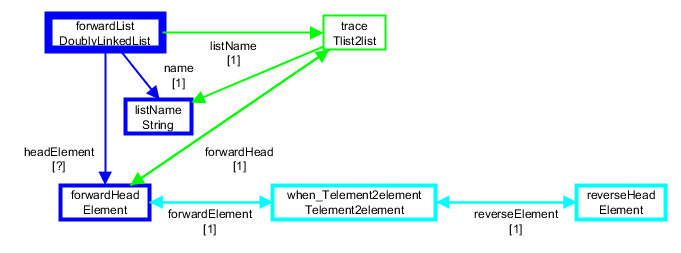
\includegraphics[width=0.45\textwidth]{List2List-trace-QVTs.png}
%	\caption{list2list trace Micro-Mapping.}
%	\label{fig:List2List-trace-QVTs}
%\end{figure}

%We have not solved the problem. We still cannot create the Tlist2list trace until we have created the Telement2element trace and vice-versa. We must be able to create at least one of the GREEN trace elements before its CYAN trace dependency.

%We need to introduce a speculative phase to the trace objects in order to break the deadlock. Figures \ref{fig:List2List-speculative-trace-QVTs}, \ref{fig:List2List-reverseList-QVTs} and \ref{fig:List2List-reverseHead-QVTs} show a sequence of compound Micro-Mappings that execute list2list speculatively.

\begin{figure}[h]
	\centering
	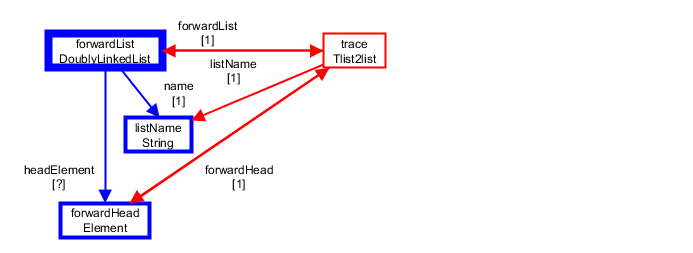
\includegraphics[width=0.45\textwidth]{List2List-speculative-trace-QVTs.png}
	\caption{list2list speculation compound Micro-Mapping in QVTs.}
	\label{fig:List2List-speculative-trace-QVTs}
\end{figure}

\begin{figure}[h]
	\centering
	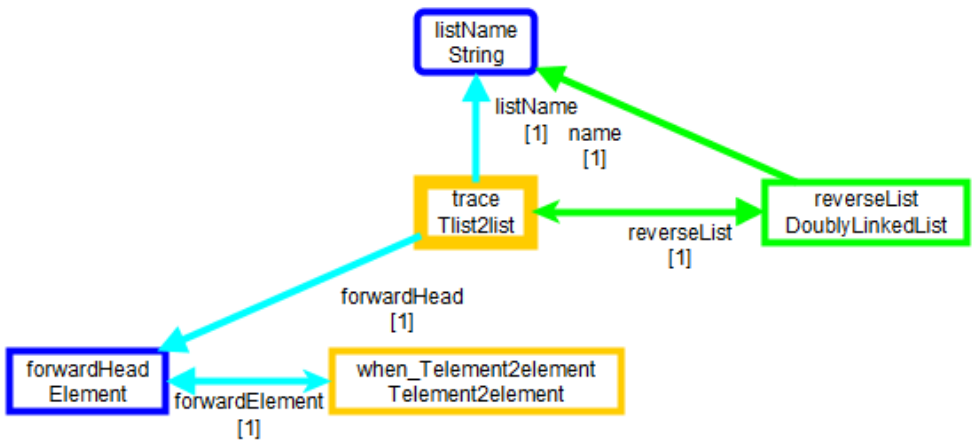
\includegraphics[width=0.45\textwidth]{List2List-reverseList-QVTs.png}
	\caption{list2list speculated compound Micro-Mapping in QVTs.}
	\label{fig:List2List-reverseList-QVTs}
\end{figure}

\begin{figure}[h]
	\centering
	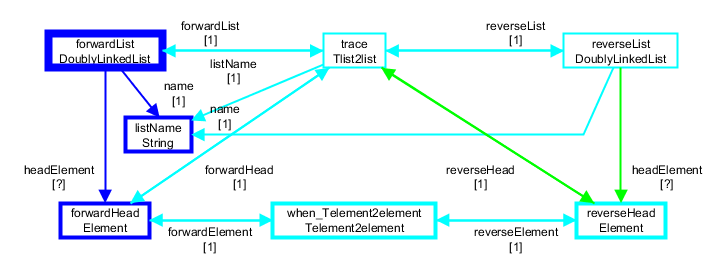
\includegraphics[width=0.45\textwidth]{List2List-reverseHead-QVTs.png}
	\caption{list2list reverseHead edges compound Micro-Mapping in QVTs.}
	\label{fig:List2List-reverseHead-QVTs}
\end{figure}

\subsubsection{Failure}

The speculation may fail, in which case Figures \ref{fig:List2List-reverseList-QVTs} and \ref{fig:List2List-reverseHead-QVTs} do not execute and no output model elements are created; the failed speculation is only visible as a still-speculating trace element in the trace model.

\subsection{ATL Execution}\label{ATL Execution}

We can now understand how ATL successfully executes the example. ATL does not perform a dependency analysis and so does not detect the difficulty. ATL just executes its rules in two stages. First all the new objects are created, then all the inter-object references are populated. ATL has therefore effectively partitioned the two list2list and element2element rules into four mini-rules list2list-create + list2list-assign, and element2element-create + element2element-assign. Executing the create mini-rules before the assign mini-rules works. This is similar to the speculation/speculated partitioning above. However ATL's partitioning is pragmatic and the successful execution fortuitous. If a more complex guard invalidates the premature creation of outputs, ATL is unable to roll-back its invalid creations.

\subsection{More Model of Computation Facilities}

Space permits only a very brief summary of the other benefits of the analyses facilitated by the Micro-Mapping Model of Computation.

\subsubsection{Multiple Heads}\label{Multiple Heads}

Micro-Mappings with multiple heads require multiple inputs and consequently incur invocation difficulties and non-linear execution performance. Analysis of the to-many metamodel relationships allows most multiple head Micro-Mappings to be realized by a single head Micro-Mapping with local rather than global loops for the other heads. This typically gives linear performance with respect to the output model size. Only genuinely Cartesian problems need incur Cartesian costs.

\subsubsection{Global optimizations}

The simple relationship between GREEN creation and CYAN use facilitates powerful global analysis. Some of these were briefly mentioned in Section \ref{Global Micro-Mapping Optimizations}

\subsubsection{Static Scheduling}

We find that most Micro-Mappings can be statically scheduled and so only a small number incur dynamic scheduling overheads at run-time.  

\subsubsection{Global Merging}

The local merging in Section~\ref{Local Merging} is heavily constrained by the requirement for a mutually shared partial truth. Once a static schedule has been established, merging can be much more aggressive. Micro-Mappings may be merged into their invokers. Predicates guaranteed by an invoker can be pruned from an invoked Micro-Mapping. 

%The never fail characteristic of the actions simplifies scheduling. In principle an unexecuted Micro-Mapping invocation can be safely retried repeatedly without any need to roll back premature partial results. In practice, a Micro-Mapping invocation failure can be related to a not-ready input so that no retry occurs until the not-ready input has been resolved. This ensures that the overheads of Micro-Mapping retries are generally below 50\%.

\subsubsection{Incremental Execution}

Execution of Micro-Mappings can be persisted as an evaluation graph comprising
\begin{itemize}
\item input nodes for each BLUE input element
\item invocation nodes for each Micro-Mapping invocation
\item BLUE-BLUE dependency edges between invocation nodes and input nodes
\item CYAN-GREEN dependency edges between consuming invocation nodes and producing invocation nodes
\end{itemize}
Each invocation node holds its prevailing GREEN state and is aware of the nodes that consume it.
The graph can be selectively re-evaluated to propagate BLUE input changes efficiently. 

%The complexity restriction on the predicates ensures that no deadlock / livelock can occur and as we have seen a mapping / Micro-Mapping that has too many dependencies can fail. At the opposite extreme, each mapping can be partitioned to contain only a single GREEN node or EDGE. This can be achieved by creating a copy of the original mapping, deleting all elements not needed by the selected GREEN element, and  recoloring all residual GREEN elements in CYAN. Figure \ref{fig:List2List-Head-QVTs} shows the minimal Micro-Mapping to perform the DoublyLinkList.headElement assignment. These maximally partitioned mappings with a single GREEN element only perform a single action, and so if there is a valid sequence of actions the maximally partitioned Micro-Mappings will execute successfully one action at a time.

%A large number of very small Micro-Mappings incurs additional overheads in their scheduling, execution and management, so we have a Goldilocks effect. We want to our Micro-Mappings to be just the right size, as large as possible to minimize overheads while avoiding livelock / deadlock hazards. We can achieve this in two stages. As soon as we have identified the minimal Micro-Mappings we may merge Micro-Mappings that share exactly the same predicates. Conversely Micro-Mappings with slightly different predicates may not be merged safely since without a global analysis, we cannot be sure that the extension of one predicate by another won't introduce a deadlock / livelock hazard via an unknown external path.

\section{Results}\label{Results}

In Figure \ref{fig:DoublyLinkedListReversalPerformance} we plot\footnote{The plots use no averaging. Single point wobbles may be due to concurrent activity. Discontinuities may be due to fortuitous cache alignment.} the performance of the DoublyLinkedListReversal transformation using a variety of transformation engines and a couple of manual implementations\footnote{Model overheads are reduced by Java generated by an EMF genmodel.}. The plot demonstrates the scalability and the underlying tooling efficiency.

\begin{figure}[h]
	\centering
	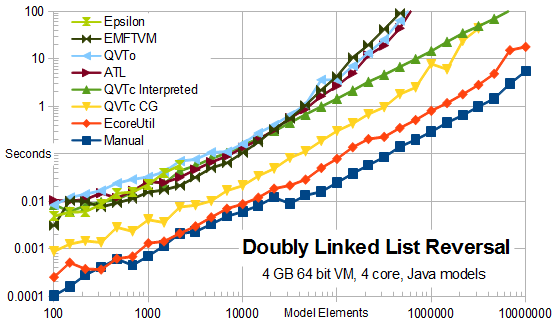
\includegraphics[width=0.48\textwidth]{DoublyLinkedListReversalPerformance.png}
	\caption{Performance of the Doubly Linked List Reversal transformation.}
	\label{fig:DoublyLinkedListReversalPerformance}
\end{figure}

Between 1000 and 50000 model elements, the top four and a half lines show superior performance for ATL and EMFTVM (the improved ATL executor) compared to Eclipse QVTo and Interpreted QVTc. However for larger models  quadratic performance, probably as a consequence of requiring a linear search of the trace to resolve output/input correspondences affects ATL, EMFTVM and QVTo. Interpreted QVTc remains linear and so at 1000000 model elements, it is 10 times faster. The performance of Epsilon for large models cannot be characterized since its half line terminates abruptly; Epsilon resolves data dependences recursively and so runs out of stack for lists longer than about 1000 elements.

The lower four lines show direct Java results, the upper two for Eclipse QVTc and QVTr, and a further two manually coded reference implementations, one using EMF extensively as a consequence of a EcoreUtil copy, and another using EMF sparingly in manual code.

QVTc and QVTr performance is almost identical since both execute the same schedule for very similar mappings. The QVTr performance is slightly worse than QVTc since the naive auto-generated trace is larger; an optimization of the auto-generated trace model will make QVTr better than QVTc. The performance almost matches EcoreUtil. Further optimizations should get much closer to the manual performance. An improved object representation could enable QVTr to outperform the manual implementation.

(The interpreted QVTc or QVTr performance may improve quite significantly once some of the static analyses for the code generated approach are exploited.)

The results demonstrate that an efficient declarative schedule can be derived automatically for a difficult dependency problem.

The results also demonstrate, unintentionally, the benefit of QVTc' explicit trace model and the consequent linear performance when an appropriate cache is synthesized for the unnavigable opposite accesses. The quadratic performance of ATL, EMFTVM and QVTo highlights an implementation deficiency that can be remedied at the expense of some extra working memory. Ensuring that the extra memory cost is modest and the additional execution time is small, probably requires similar static compile-time or load-time analyses to those performed by Eclipse QVTd.

The code and results for this example are available in the tests/org.eclipse.qvtd.doc.exe2016.tests plugin of the https://git.eclipse.org/r/mmt/org.eclipse.qvtd GIT repository. Significant bugs in Eclipse QVTd were fixed to support this example. These fixes should be available in the Oxygen M2 milestone build in mid September 2016.

%This example was also attempted with Eclipse QVTr, but unfortunately the partitioning algorithm neglected to partition to respect a Class dependency; the resulting code compiled and executed but produced no output. The corresponding QVTc exposed the dependency as a Property dependency and the partitioning succeeded. Hopefully the partitioning bug will be fixed in time for the camera ready copy. The QVTr performance is likely to be very similar to the QVTc performance.

%These results were produced before the write up of Micro-Mapping partitioning revealed the need for speculative trace creation. The results for at least ATL and QVTc are therefore based on an unsound execution model that all objects can be created early. 

\section{Related Work}\label{Related Work}

Scheduling and particularly static scheduling has been a rich research topic with provision of optimized schedules recognized as a computationally hard problem. The many works of the Ptolemy group \cite{dataflow} that build upon \cite{sdf} has been a strong background influence. However the appreciation that metamodels impose such strong constraints that sensible schedules can be produced rapidly for declarative transformations appears to be novel.

The Graph Transformation community has been very active in providing a rigorous foundation for graph mappings. Sadly the QVT specification ignored this important work, preferring instead to define the semantics of the QVTr transformation language using an incomplete exposition of a transformation of QVTr written in an untested QVTr to another language (QVTc) that has at best informal semantics. The utility and power of the QVTs graphical Micro-Mapping and its Model of Computation may begin to bridge the gap between these two communities. The automated coloring in QVTs is inspired by Henshin's \cite{Henshin} manual use of colors to denote create/delete/no-change in endogenous transformations. The reification of the QVTc traceability element mirrors the evolution operators in UMLX~\cite{UMLX} for heterogeneous transformations.

Active Operations~\cite{Jouault-ActiveOperations} also reify mappings 
%at run-time
to persist the state necessary for incremental execution. Micro-Mappings similarly support incremental execution, but their primary rationale is to be a deadlock-free unit of computation.

% An example of a floating figure using the graphicx package.
% Note that \label must occur AFTER (or within) \caption.
% For figures, \caption should occur after the \includegraphics.
% Note that IEEEtran v1.7 and later has special internal code that
% is designed to preserve the operation of \label within \caption
% even when the captionsoff option is in effect. However, because
% of issues like this, it may be the safest practice to put all your
% \label just after \caption rather than within \caption{}.
%
% Reminder: the "draftcls" or "draftclsnofoot", not "draft", class
% option should be used if it is desired that the figures are to be
% displayed while in draft mode.
%
%\begin{figure}[!t]
%\centering
%\includegraphics[width=2.5in]{myfigure}
% where an .eps filename suffix will be assumed under latex, 
% and a .pdf suffix will be assumed for pdflatex; or what has been declared
% via \DeclareGraphicsExtensions.
%\caption{Simulation results for the network.}
%\label{fig_sim}
%\end{figure}

% Note that the IEEE typically puts floats only at the top, even when this
% results in a large percentage of a column being occupied by floats.


% An example of a double column floating figure using two subfigures.
% (The subfig.sty package must be loaded for this to work.)
% The subfigure \label commands are set within each subfloat command,
% and the \label for the overall figure must come after \caption.
% \hfil is used as a separator to get equal spacing.
% Watch out that the combined width of all the subfigures on a 
% line do not exceed the text width or a line break will occur.
%
%\begin{figure*}[!t]
%\centering
%\subfloat[Case I]{\includegraphics[width=2.5in]{box}%
%\label{fig_first_case}}
%\hfil
%\subfloat[Case II]{\includegraphics[width=2.5in]{box}%
%\label{fig_second_case}}
%\caption{Simulation results for the network.}
%\label{fig_sim}
%\end{figure*}
%
% Note that often IEEE papers with subfigures do not employ subfigure
% captions (using the optional argument to \subfloat[]), but instead will
% reference/describe all of them (a), (b), etc., within the main caption.
% Be aware that for subfig.sty to generate the (a), (b), etc., subfigure
% labels, the optional argument to \subfloat must be present. If a
% subcaption is not desired, just leave its contents blank,
% e.g., \subfloat[].


% An example of a floating table. Note that, for IEEE style tables, the
% \caption command should come BEFORE the table and, given that table
% captions serve much like titles, are usually capitalized except for words
% such as a, an, and, as, at, but, by, for, in, nor, of, on, or, the, to
% and up, which are usually not capitalized unless they are the first or
% last word of the caption. Table text will default to \footnotesize as
% the IEEE normally uses this smaller font for tables.
% The \label must come after \caption as always.
%
%\begin{table}[!t]
%% increase table row spacing, adjust to taste
%\renewcommand{\arraystretch}{1.3}
% if using array.sty, it might be a good idea to tweak the value of
% \extrarowheight as needed to properly center the text within the cells
%\caption{An Example of a Table}
%\label{table_example}
%\centering
%% Some packages, such as MDW tools, offer better commands for making tables
%% than the plain LaTeX2e tabular which is used here.
%\begin{tabular}{|c||c|}
%\hline
%One & Two\\
%\hline
%Three & Four\\
%\hline
%\end{tabular}
%\end{table}


% Note that the IEEE does not put floats in the very first column
% - or typically anywhere on the first page for that matter. Also,
% in-text middle ("here") positioning is typically not used, but it
% is allowed and encouraged for Computer Society conferences (but
% not Computer Society journals). Most IEEE journals/conferences use
% top floats exclusively. 
% Note that, LaTeX2e, unlike IEEE journals/conferences, places
% footnotes above bottom floats. This can be corrected via the
% \fnbelowfloat command of the stfloats package.




\section{Conclusion}\label{Conclusions}

We have introduced the Micro-Mapping Model of Computation and shown how it supports efficient declarative schedules for Eclipse QVTc and QVTr.

We used the Micro-Mapping Model of Computation to demonstrate the need for speculative creation of trace objects.

We have shown how a graphical presentation of metamodel and dependency analyses tames the naive inefficiencies of a declarative schedule.

We have introduced the first implementation of the QVTc specification.

We have presented the first results for a QVTr implementation using a direct code generator.

We have mentioned some future works. Many more optimizations to do.
%that with a planned schedule declarative transformations do not have to be slower than imperative transformations.



% conference papers do not normally have an appendix


% use section* for acknowledgment
\section*{Acknowledgment}

The authors would like to thank Adolfo Sanchez-Barbudo Herrera, Horacio Hoyos Rodriguez, Dimitris Kolovos and Richard Paige for helpful discussions about declarative scheduling approaches. Horacio prepared some of the results and prototyped some of the scheduler algorithms.

% trigger a \newpage just before the given reference
% number - used to balance the columns on the last page
% adjust value as needed - may need to be readjusted if
% the document is modified later
%\IEEEtriggeratref{8}
% The "triggered" command can be changed if desired:
%\IEEEtriggercmd{\enlargethispage{-5in}}

% references section

% can use a bibliography generated by BibTeX as a .bbl file
% BibTeX documentation can be easily obtained at:
% http://mirror.ctan.org/biblio/bibtex/contrib/doc/
% The IEEEtran BibTeX style support page is at:
% http://www.michaelshell.org/tex/ieeetran/bibtex/
%\bibliographystyle{IEEEtran}
% argument is your BibTeX string definitions and bibliography database(s)
%\bibliography{IEEEabrv,../bib/paper}
%
% <OR> manually copy in the resultant .bbl file
% set second argument of \begin to the number of references
% (used to reserve space for the reference number labels box)
\begin{thebibliography}{1}

\bibitem{dataflow}
Bhattacharyya, S., Murthy, P., Lee, E.: Software synthesis from dataflow graphs, Kluwer Academic Press, Norwell, MA, 1996

\bibitem {Henshin}
Biermann, E., Ermel, C., Schmidt, J., Warning, A.:
Visual Modeling of Controlled EMF Model Transformation using HENSHIN
Proceedings of the Fourth International Workshop on Graph-Based Tools, GraBaTs 2010.

\bibitem{Jouault-ActiveOperations}
Jouault, F., Beaudoux, O.:
On the Use of Active Operations for Incremental Bidirectional Evaluation of OCL
15th International Workshop on OCL and Textual Modeling, Ottawa, 2015

\bibitem{sdf}
Lee, E., Messerschmitt, D.: Synchronous data flow, Proceedings of the IEEE, 1987

\bibitem{moc}
Lee, E., Sangiovanni-Vincentelli, A.: Comparing models of computation, Proceedings of the 1996 IEEE/ACM international conference on Computer-aided design

\bibitem{QVT-1.3}
OMG. Meta Object Facility (MOF) 2.0 Query/View/Transformation Specification, Version 1.3.
OMG Document Number: ptc/16-06-03, June 2016.

\bibitem{UMLX}
Willink, E: UMLX : A Graphical Transformation Language for MDA
Model Driven Architecture: Foundations and Applications, MDAFA 2003, Twente, June 2003.
\url{http://eclipse.org/gmt/umlx/doc/MDAFA2003-4/MDAFA2003-4.pdf}

\bibitem {ya3qvt}
Willink, E.:
Yet Another Three QVT Languages.
ICMT 2013 (2013)

\bibitem{Eclipse-ATL}
Eclipse ATL Project.\\
\url{https://projects.eclipse.org/projects/modeling.mmt.atl}

\bibitem{Eclipse-EMF}
Eclipse EMF Project.\\
\url{https://projects.eclipse.org/projects/modeling.emf.emf}

\bibitem{Eclipse-OCL}
Eclipse OCL Project.\\
\url{https://projects.eclipse.org/projects/modeling.mdt.ocl}

\bibitem{Eclipse-QVTd}
Eclipse QVT Declarative Project.\\
\url{https://projects.eclipse.org/projects/modeling.mmt.qvtd}
\end{thebibliography}




% that's all folks
\end{document}


